\documentclass[11pt,a4paper]{article}

% ── Font: Times-like serif (newtxtext + newtxmath) ──────────────────────────
\usepackage[T1]{fontenc}
\usepackage{newtxtext}
\usepackage{newtxmath}

% ── Layout: tight but readable. 6 pages of body is the hard cap. ────────────
\usepackage[margin=2.2cm, top=2.2cm, bottom=2.2cm]{geometry}
\usepackage{setspace}
\setstretch{1.08}
\setlength{\parskip}{4pt}
\setlength{\parindent}{0pt}

% ── Packages ─────────────────────────────────────────────────────────────────
\usepackage{graphicx}
\usepackage{booktabs}
\usepackage{tabularx}
\usepackage{array}
\usepackage{amsmath}
\usepackage{xcolor}
\usepackage{float}
\usepackage{caption}
\usepackage[hidelinks, colorlinks=true, linkcolor=black, citecolor=blue!60!black, urlcolor=blue!60!black]{hyperref}
\usepackage{enumitem}
\usepackage{needspace}
\setlist{itemsep=1pt, parsep=0pt, topsep=2pt, leftmargin=1.3em}

% Unequal-width X columns for tabularx (sum of hsize multipliers must equal
% the number of X-columns in the table — 3 in our risk-register table).
\newcolumntype{Y}[1]{>{\hsize=#1\hsize\linewidth=\hsize}X}

% ── Figures path ─────────────────────────────────────────────────────────────
\graphicspath{{figures/}}

% ── Section formatting: compact ─────────────────────────────────────────────
\usepackage{titlesec}
\titlespacing*{\section}{0pt}{10pt}{4pt}
\titlespacing*{\subsection}{0pt}{6pt}{2pt}
\titleformat{\section}{\large\bfseries}{\thesection.}{0.5em}{}
\titleformat{\subsection}{\normalsize\bfseries}{\thesubsection}{0.5em}{}

% ── Captions ─────────────────────────────────────────────────────────────────
\captionsetup{font=small, skip=4pt, labelfont=bf, justification=justified, singlelinecheck=false}
\captionsetup[table]{position=above, skip=3pt}
\captionsetup[figure]{position=below, skip=4pt}

% ── Header/footer ────────────────────────────────────────────────────────────
\usepackage{fancyhdr}
\pagestyle{fancy}
\fancyhf{}
\fancyfoot[C]{\thepage}
\renewcommand{\headrulewidth}{0pt}
\fancypagestyle{plain}{\fancyhf{}\fancyfoot[C]{\thepage}\renewcommand{\headrulewidth}{0pt}}

% ── Inline code ──────────────────────────────────────────────────────────────
\newcommand{\code}[1]{\texttt{\small #1}}

% ── Table of contents styling ────────────────────────────────────────────────
% Paper convention: "Contents" centered in moderate bold, no decorative rule.
% Section entries in regular weight (not bold) so the page-number rail does
% not compete visually with the section titles. Subsections indented and
% slightly smaller. Page numbers right-aligned, subtle dot leaders.
\usepackage{tocloft}
\renewcommand{\contentsname}{Contents}
\renewcommand{\cfttoctitlefont}{\hspace*{\fill}\Large\bfseries}
\renewcommand{\cftaftertoctitle}{\hspace*{\fill}\par\vspace{18pt}}
\setlength{\cftbeforesecskip}{7pt}
\setlength{\cftbeforesubsecskip}{2pt}
\setlength{\cftsecindent}{0pt}
\setlength{\cftsecnumwidth}{1.8em}
\setlength{\cftsubsecindent}{1.8em}
\setlength{\cftsubsecnumwidth}{1.6em}
% Section number + title: roman, normal size. Subsection: small.
\renewcommand{\cftsecfont}{\normalsize}
\renewcommand{\cftsubsecfont}{\small}
\renewcommand{\cftsecpagefont}{\normalsize}
\renewcommand{\cftsubsecpagefont}{\small}
% Dot leaders: present but light, evenly spaced.
\renewcommand{\cftsecleader}{\cftdotfill{\cftsecdotsep}}
\renewcommand{\cftsecdotsep}{5}
\renewcommand{\cftdotsep}{5}

% ── Widow/orphan control ────────────────────────────────────────────────────
\widowpenalty=10000
\clubpenalty=10000
\displaywidowpenalty=10000
\raggedbottom
\renewcommand{\topfraction}{0.92}
\renewcommand{\bottomfraction}{0.85}
\renewcommand{\textfraction}{0.06}
\renewcommand{\floatpagefraction}{0.7}
\frenchspacing

% ══════════════════════════════════════════════════════════════════════════════
\begin{document}

% ── Title page ───────────────────────────────────────────────────────────────
\begin{titlepage}
    \centering
    \vspace*{3cm}

    {\Huge\bfseries Hourly Electricity Load\\[8pt] Forecasting in Production\par}

    \vspace{1.2cm}

    {\Large An End-to-End MLOps Proof of Concept\\[4pt]
    with Drift Monitoring, Quantile Intervals, and a Feature Store\par}

    \vspace{2.5cm}

    {\large
    \begin{tabular}{c}
        Samuel Braun, 20250355\\
        Margarida Quintino, 20250411\\
        Giosu\`e Morelli, 20250472\\
    \end{tabular}
    \par}

    \vspace{1.6cm}

    {\large MLOps -- 2025/2026\par}

    \vfill

    {\large NOVA Information Management School\par}
    {\large June 2026\par}
\end{titlepage}

% ── Table of Contents (does not count toward the 6-page body) ───────────────
\clearpage
\pagenumbering{roman}
\setcounter{page}{1}
{\renewcommand{\baselinestretch}{1.0}\normalsize
\tableofcontents}
\clearpage
\pagenumbering{arabic}
\setcounter{page}{1}

% ══════════════════════════════════════════════════════════════════════════════
\section{Problem and Objective}
% ══════════════════════════════════════════════════════════════════════════════

Short-horizon electricity load forecasting drives day-ahead generation scheduling, reserve sizing, and intraday market clearing. A 24-hour-ahead forecast at hourly resolution has to be accurate enough for unit-commitment decisions and calibrated enough that downstream optimisation can reason about uncertainty. The point-forecasting problem itself is largely solved for national load: gradient-boosted trees on lag and calendar features reach sub-2\% MAPE without much effort. The harder problem, and the one this project tackles, is the surrounding system. We needed a model whose training run is reproducible from a clean clone, whose lineage stays traceable through to the deployed prediction, whose inputs are monitored for distribution shift, and whose stack stays serviceable as dependencies age.

The system-level objectives are: (i) data-quality gates that abort the pipeline on schema or range violations before a bad batch reaches training; (ii) a feature store that serves identical definitions at training and inference time; (iii) experiment tracking with a single registered model, promoted by stage rather than by file path; (iv) prediction intervals calibrated to a nominal 80\% level; (v) a drift monitor that fires on real distribution shift and quiesces when it passes; and (vi) CI that gates every commit on lint, type, and test checks.

% ══════════════════════════════════════════════════════════════════════════════
\section{Dataset and Metrics}
% ══════════════════════════════════════════════════════════════════════════════

We use the Open Power System Data hourly time series for Germany~\cite{opsd2020}, 50{,}401 hourly observations from 2015-01-01 to 2020-09-30, sourced from the ENTSO-E Transparency Platform~\cite{entsoe2024transparency}. The target is total German load (\code{load\_mw}); wind and solar generation enter as exogenous variables. The temporal partition is a strict chronological 70/15/15 split: train 2015--2018, validation 2019, test 2020. Random shuffling is prohibited; permuting a time series before splitting leaks future observations into training and silently inflates validation metrics. The 2020 test partition is retained on purpose so that it contains the COVID-19 lockdown, a known structural break that lets the drift pipeline be empirically falsified (Section~5).

Point-forecast quality is reported as MAPE (primary, scale-invariant, the load-forecasting convention~\cite{hong2016probabilistic}) and RMSE in megawatts. MAPE is known to bias toward under-forecasting; we accept it because German load never approaches zero and the seasonal-naive baseline acts as an implicit scaled comparator (equivalent in spirit to MASE). Walk-forward cross-validation reports MAPE mean and standard deviation across four expanding-window folds. Interval quality is empirical coverage against the 80\% nominal level and the average width in MW. Distribution shift is the average Wasserstein drift score under Evidently; concept drift is monthly test MAPE against a 1.5$\times$ median-of-non-perturb-months baseline. The 1.5$\times$ multiplier is a tuned heuristic, not a statistical bound, but April 2020 is the only month that would breach it under any multiplier between 1.3 and 2.0, so the conclusion is not sensitive to the exact value.

% ══════════════════════════════════════════════════════════════════════════════
\section{System Architecture and Technology}
% ══════════════════════════════════════════════════════════════════════════════

Eight Kedro pipelines move data from the raw CSV to the registered Production model, each owning a single concern and writing into the next layer of the Kedro data catalog (Table~\ref{tab:pipelines}). The numbering follows the standard Kedro eight-layer data-engineering convention: 01~raw, 02~intermediate, 03~primary, 04~feature, 05~model-input, 06~models, 07~model-output, 08~reporting; layer~03 is reserved by the convention and unused here because no aggregation step sits between cleaning and feature engineering. The serving stack (FastAPI, Streamlit, Feast, MLflow) sits on top of those outputs and is the only surface external consumers see.

\begin{table}[H]
\centering
\small
\begin{tabularx}{\linewidth}{@{}l l X@{}}
\toprule
\textbf{Pipeline} & \textbf{Layer in $\rightarrow$ out} & \textbf{Owns} \\
\midrule
\code{data\_quality}\textsuperscript{$\dagger$}    & 01 $\rightarrow$ 08 & Great Expectations v1 suite (10 expectations); validation report \\
\code{data\_cleaning}          & 01 $\rightarrow$ 02 & Timestamp normalisation, gap fill, IQR outliers \\
\code{data\_feat\_engineering} & 02 $\rightarrow$ 04 & Lag features, rolling stats, calendar, Fourier \\
\code{data\_split}             & 04 $\rightarrow$ 05 & Strict chronological train/val/test split \\
\code{model\_train}            & 05 $\rightarrow$ 06 & Three candidates, MLflow logging, SHAP \\
\code{model\_selection}\textsuperscript{$\ddagger$} & 06 $\rightarrow$ \textit{registry} & Promote winner None $\to$ Staging $\to$ Production \\
\code{model\_predict}          & 05 $\rightarrow$ 07 & Load by registry stage, predict on test \\
\code{data\_drifts}            & 07 $\rightarrow$ 08 & Univariate + concept drift, dual-window \\
\bottomrule
\end{tabularx}
\caption{Kedro pipelines and their catalog layers. $\dagger$~writes a validation report rather than a transformed dataset. $\ddagger$~registry stage transition, no data layer.}
\label{tab:pipelines}
\end{table}

\textbf{Project planning.} Work was organized into three two-week sprints aligned with the course schedule. Sprint~1 covered dataset selection, the Great Expectations suite, feature engineering, and MLflow experiment tracking. Sprint~2 covered Kedro modularization across the eight leaf pipelines, the GitHub Actions CI matrix on Python 3.11 and 3.12, the multi-stage Docker images, and the FastAPI serving layer. Sprint~3 covered the dual-window drift detector, SHAP explainability, the Streamlit dashboard, split-conformal calibration of the prediction intervals, and this report. Each sprint produced a runnable end-to-end version of the system; later sprints replaced placeholders rather than adding new layers, which kept the pipeline graph close to deliverable throughout.

\textbf{Technology stack.} Orchestration: Kedro 0.19 with kedro-mlflow and kedro-viz. Tracking and registry: MLflow 2.15. Feature store: Feast 0.58, with offline Parquet and a SQLite online store. Data quality: Great Expectations 1.x. Drift: Evidently 0.7. Models: LightGBM 4.6, Prophet 1.1, and a seasonal-naive baseline. Explainability: SHAP TreeExplainer. Serving: FastAPI plus Uvicorn in a multi-stage Docker image. Dashboard: Streamlit. CI: GitHub Actions running Ruff, mypy, pytest, and a Kedro registry smoke check on Python 3.11 and 3.12. Pre-commit hooks gate lint, format, secrets, and large files. Three components depart from the literal handout for maintenance reasons: Feast replaces Hopsworks (runs from a clean clone with no hosted account), Evidently replaces NannyML (a permitted alternative in the handout), and Great Expectations 1.x replaces 0.18 (which is in deprecation). A pinned package list with exact versions is in Annex~G.

\textbf{Feature store role.} Feast is the single source of truth for feature definitions across training and serving. The \code{feast-publish} step reads the schema in \code{feature\_store/feature\_repo/electricity.py}, registers the layer-04 Parquet as the offline source, and materialises the latest values into a SQLite online store the FastAPI service reads from at inference time. The shared definition file closes the training/serving skew risk listed in Section~7.

\textbf{Training/serving separation.} The inference image excludes Kedro, SHAP, Evidently, and Great Expectations. The \code{QuantileLGBM} pyfunc that MLflow deserialises at serving time lives in its own \code{serving} module, so cloudpickle does not transitively pull Kedro into the API. The API addresses the model by registry name and stage, never by file path, so promotions and rollbacks are registry operations rather than image rebuilds.

\textbf{Reproduction.} A clean clone reaches a running stack in five \code{make} targets: \code{install} (venv + editable install), \code{download-data} (OPSD CSV into \code{data/01\_raw/}), \code{run} (all eight pipelines, $\sim$3 min), \code{feast-publish} (apply and materialise the Feast store), and \code{serve} (Docker Compose: MLflow 5000, FastAPI 8000, Streamlit 8501). Every MLflow run logs a SHA-256 hash of the training Parquet, so identical inputs produce identical hashes and silent input changes show up in the comparison view. The system shape reflects findings that glue dominates the model in deployed ML~\cite{sculley2015hidden, paleyes2022challenges} and that data and production-readiness checks belong inside the pipeline~\cite{schelter2018datavalidation, breck2017tests}.

% ══════════════════════════════════════════════════════════════════════════════
\section{Methodology and Results}
% ══════════════════════════════════════════════════════════════════════════════

\textbf{Features.} A 39-predictor representation in five families: 8 lags (\code{1,2,3,6,12,24,48,168}h), 8 rolling statistics (mean and standard deviation over 6/12/24/168h windows, each preceded by \code{shift(1)} so that the value at time $t$ does not contain its own predictor), 9 calendar variables (hour, day-of-week, day-of-year, month, week-of-year, weekend flag, season, holiday flag, working-day flag), 12 Fourier terms (sine and cosine pairs at the 24h and 168h periods, harmonic orders 1--3), and 2 exogenous series (wind and solar generation). Lag and rolling features are computed inside each split, never on the concatenated frame.

\textbf{Models.} Three candidates following the M4 recommendation~\cite{makridakis2020m4} that any method be benchmarked against a non-parametric and a statistical baseline: seasonal-naive at $T{-}168$h as the falsifiability floor, Prophet~\cite{taylor2018prophet} as a structural decomposition baseline, and LightGBM~\cite{ke2017lightgbm} as the production candidate. LightGBM is evaluated under expanding-window walk-forward cross-validation with four folds; per-fold details are in Annex~A.

\textbf{Prediction intervals.} Two auxiliary LightGBM heads at $\alpha = 0.1$ and $\alpha = 0.9$ produce raw quantile bounds. Vanilla quantile regression undercovers on heteroscedastic targets, so we apply split-conformal calibration~\cite{romano2019cqr, angelopoulos2021gentle}: on the validation calibration set we compute the non-conformity score $s_i = \max(\hat{q}_{0.1}(x_i) - y_i,\, y_i - \hat{q}_{0.9}(x_i))$ and widen every interval at inference by the $(1-\alpha)$ empirical quantile of $\{s_i\}$. The three heads ship as a single MLflow pyfunc, so the API does one deserialisation per worker.

\textbf{Results.} The deployed LightGBM reaches 1.02\% test MAPE on the 2020 test partition (Jan--Sep, including the COVID-19 lockdown), about six times better than the seasonal-naive baseline and seven times better than Prophet on the validation set (Figure~\ref{fig:model_comparison}, Table~\ref{tab:headline}). Validation coverage under split-conformal is the nominal 80.0\% by construction. Test coverage is 73.1\%: calibration tuned on 2019 (a quiet year) and tested on 2020 (the most abnormal year in the dataset) under-covers by design, because the COVID-19 lockdown violates the exchangeability assumption split-conformal relies on. We chose the split to expose this failure mode rather than hide it. The Adaptive Conformal Inference baseline~\cite{gibbs2021aci} that runs alongside every prediction recovers 80.1\% test coverage by widening the offset from 201~MW to 238~MW over the test window. We keep the simpler split-conformal contract deployed and log ACI as a sibling MLflow run, because the resulting coverage gap is itself a useful drift signal and promoting ACI is a few lines of change inside the wrapper.

\begin{figure}[H]
    \centering
    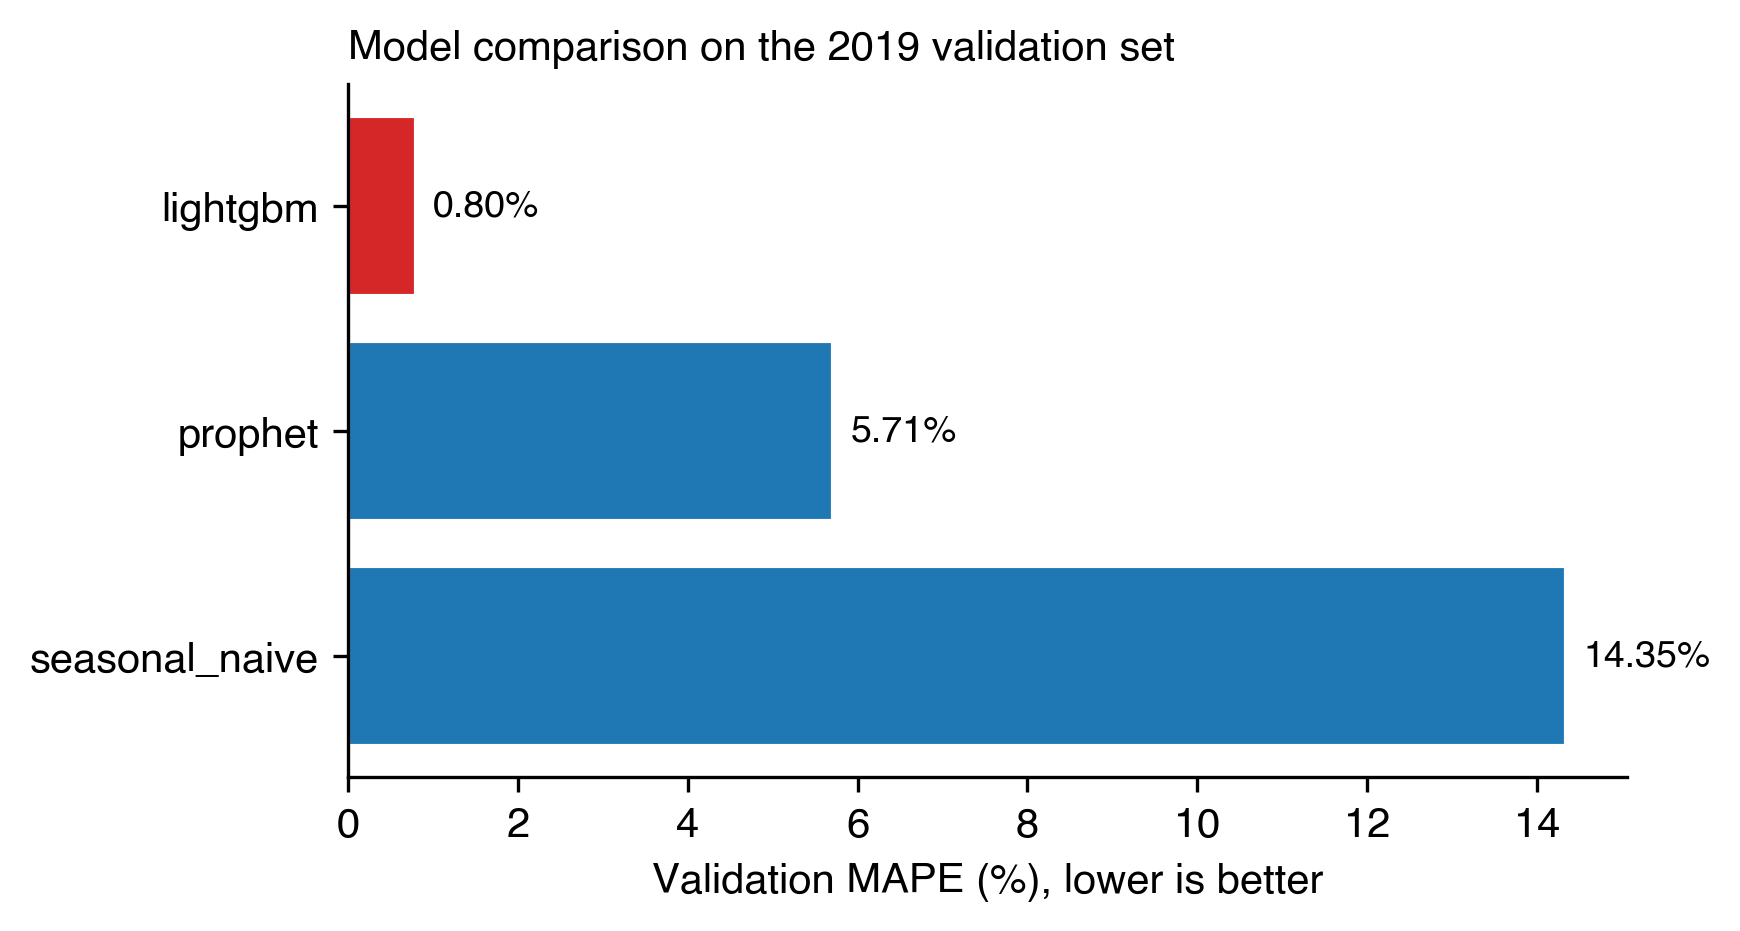
\includegraphics[width=0.55\linewidth]{model_comparison.png}
    \caption{Validation MAPE per candidate, lower is better.}
    \label{fig:model_comparison}
\end{figure}

\begin{table}[H]
\centering
\small
\begin{tabularx}{\linewidth}{@{}l *{5}{>{\centering\arraybackslash}X}@{}}
\toprule
\textbf{Model} & \textbf{Val MAPE} & \textbf{Val RMSE} & \textbf{Test MAPE} & \textbf{Val coverage} & \textbf{Test coverage} \\
\midrule
Seasonal Naive ($T{-}168$h)   & 4.74\% & 4{,}465~MW & ---     & ---    & ---    \\
Prophet (multiplicative)      & 5.71\%  & 4{,}061~MW  & ---     & ---    & ---    \\
\textbf{LightGBM (split-conformal)} & \textbf{0.80\%} & \textbf{570~MW} & \textbf{1.02\%} & \textbf{80.0\%} & \textbf{73.1\%} \\
LightGBM + ACI ($\gamma=0.005$) & ---   & ---         & 1.02\%  & ---    & 80.1\% \\
\bottomrule
\end{tabularx}
\caption{Point-forecast and interval-coverage results. Walk-forward CV: $0.93\% \pm 0.15\%$, 4 folds.}
\label{tab:headline}
\end{table}

\textbf{What the model relies on.} SHAP TreeExplainer attributions~\cite{lundberg2017shap} on a 300-sample validation slice (Annex~B) put the 24-hour lag first at a mean absolute SHAP of 4{,}812~MW, followed by the 168-hour lag at 1{,}706~MW and the 24-hour rolling mean at 887~MW. Calendar features (hour-of-day, working-day indicator) sit in the second tier; wind and solar generation rank lower than we expected at the 24-hour horizon. This is more or less the classical autocorrelation picture for national load: yesterday at the same hour is the strongest predictor, with last week's hour as a secondary anchor. The same effect is why a strict $T{-}168$h seasonal-naive already reaches 4.74\% validation MAPE without any model at all, and is the reason Prophet sits at 5.71\% despite its richer trend decomposition: at this horizon, the autoregressive structure dominates calendar effects.

\textbf{Stability across time.} Walk-forward cross-validation with four expanding-window folds gives a per-fold MAPE mean of 0.93\% with a standard deviation of 0.15 percentage points (Figure~\ref{fig:cv_folds}). The earliest fold is the hardest, with only a year of training data behind it; performance settles below the 1\% mark from the half-data fold onward. The dispersion is too small to change which model wins, but big enough that we put it on the model card next to the headline MAPE rather than hide it.

\begin{figure}[H]
    \centering
    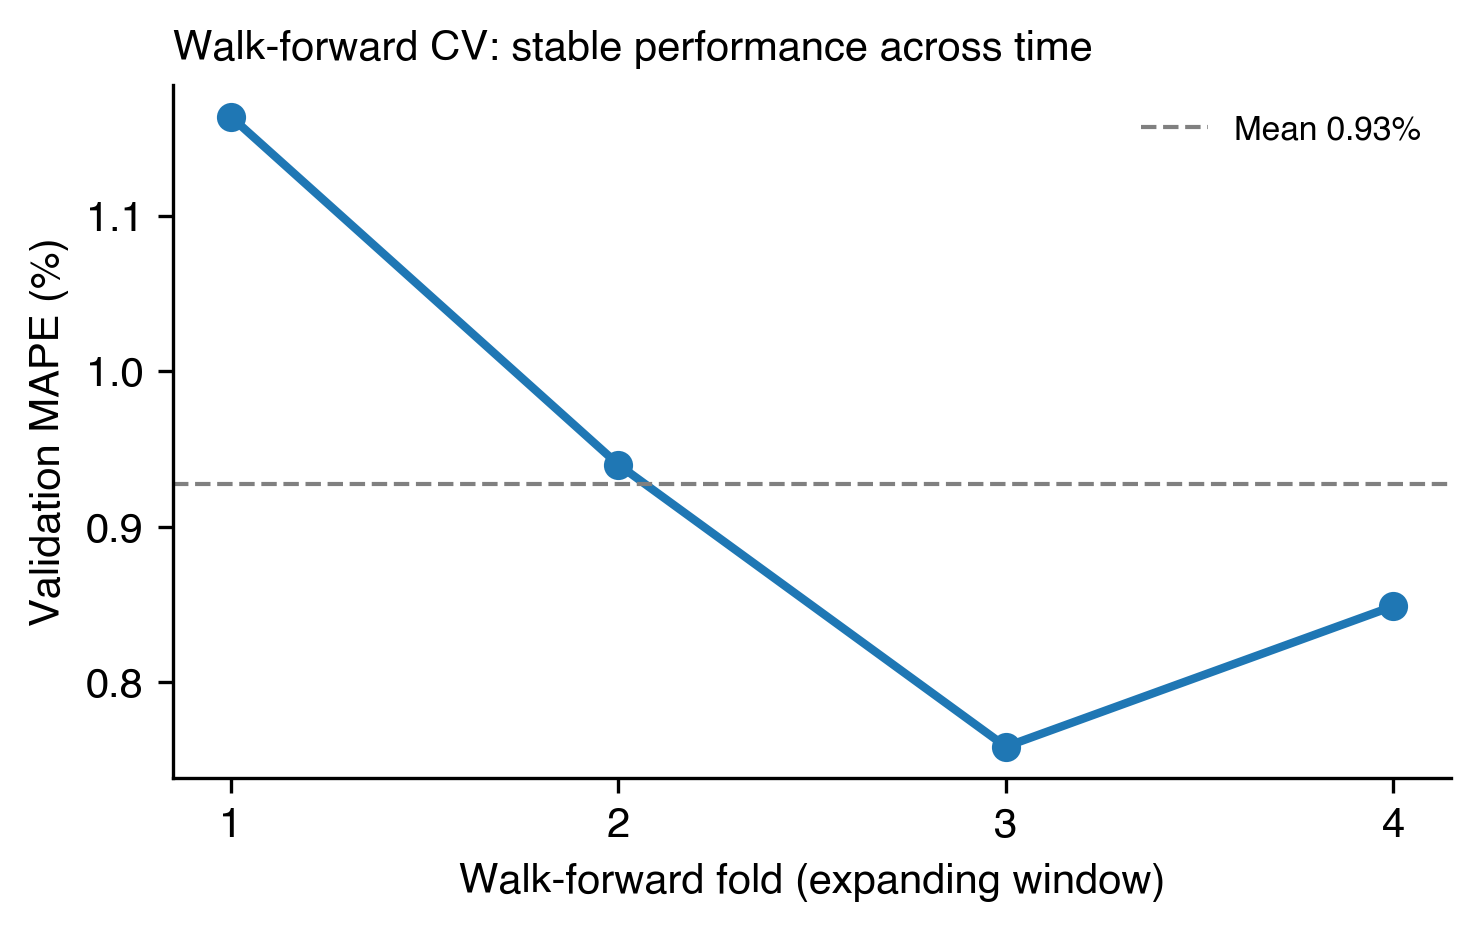
\includegraphics[width=0.5\linewidth]{cv_folds.png}
    \caption{Walk-forward validation MAPE per fold.}
    \label{fig:cv_folds}
\end{figure}

% ══════════════════════════════════════════════════════════════════════════════
\needspace{30\baselineskip}
\section{Drift Monitoring}
\label{sec:drift}
% ══════════════════════════════════════════════════════════════════════════════

A drift monitor whose output never changes adds no diagnostic information~\cite{rabanser2019failing}. The drift pipeline therefore runs Evidently on \emph{two} current-data windows from the same 2019 H1 reference: a within-distribution control window (2019-07 to 2019-12, no drift expected) and the COVID-19 lockdown window (2020-03 to 2020-05, drift expected). The control already crosses Evidently's default 0.10 Wasserstein threshold on ordinary seasonal variation (average score 0.22, 13 of 15 features flagged); the lockdown crosses it at 0.66 across all 15 features (Figure~\ref{fig:drift}). The threshold is too sensitive for raw seasonal data, so the signal we actually rely on is the threefold separation in magnitude between the two windows, not the binary alert.

Concept drift is monitored separately, on the model output rather than its inputs, as monthly test MAPE against a 1.5$\times$ median-of-non-perturb-months baseline. April 2020 is the only month that breaches the threshold and would trigger automated retraining in a real deployment. The detector then quiets down once the lockdown effect passes, which is what stops it from becoming the kind of always-alerting monitor that operators eventually start ignoring.

\begin{figure}[H]
    \centering
    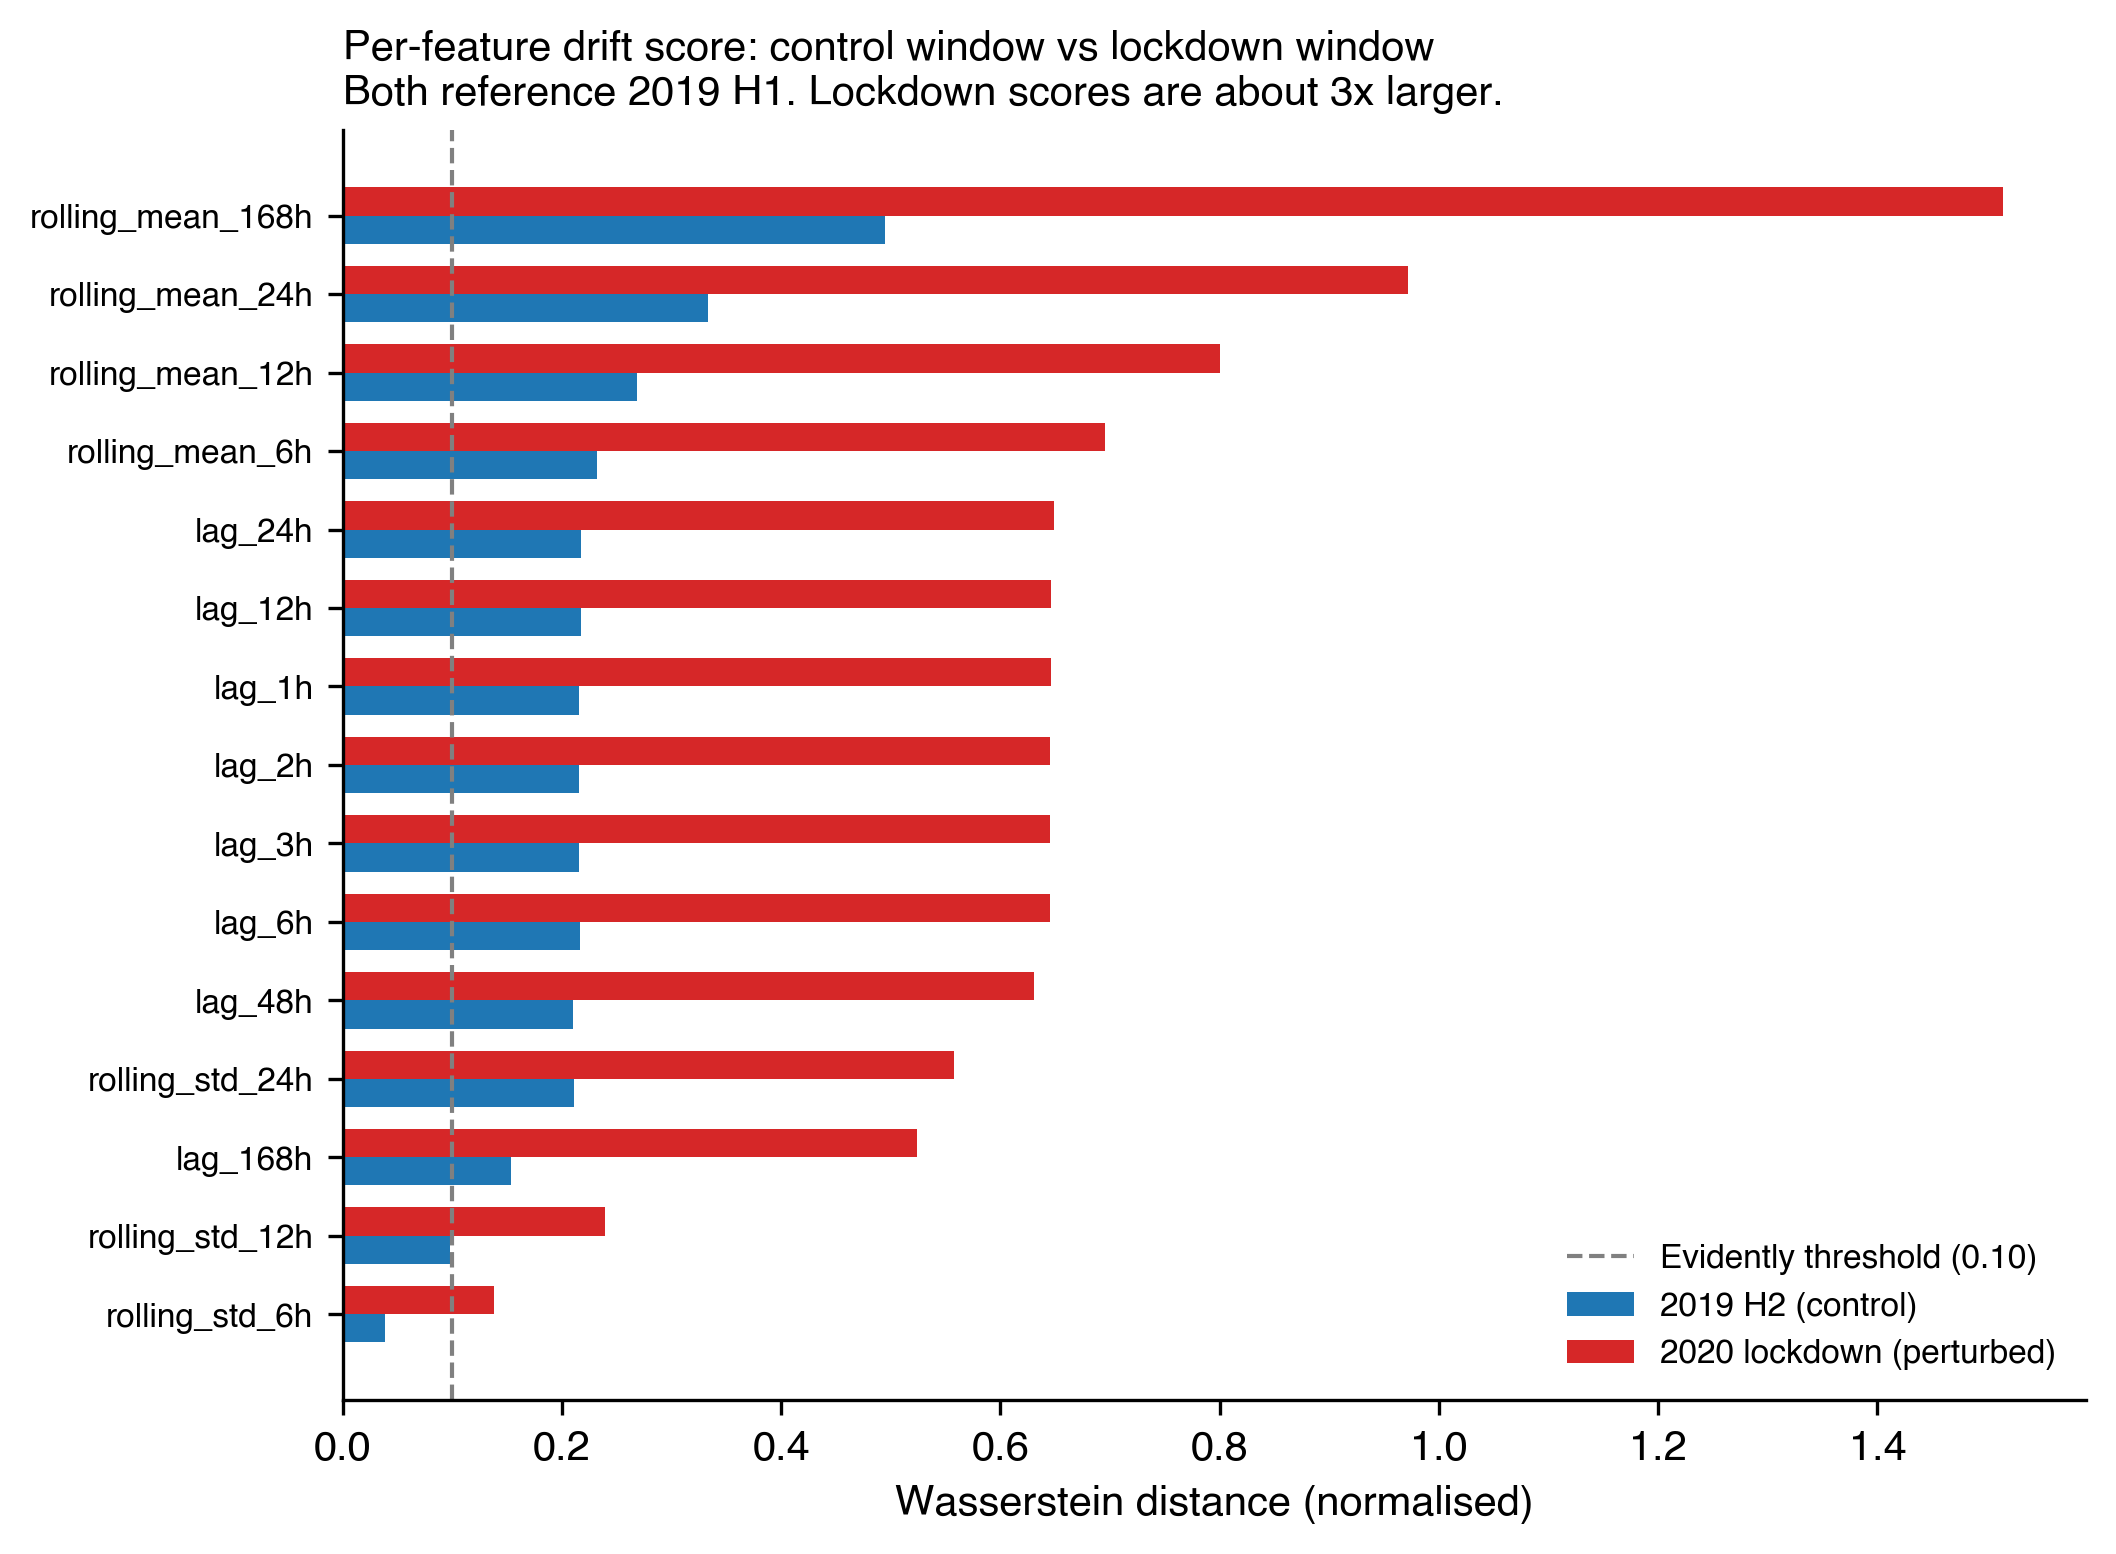
\includegraphics[width=0.72\linewidth]{drift_comparison.png}
    \caption{Per-feature Wasserstein drift, control vs lockdown, against the 2019 H1 reference. Dashed: Evidently 0.10 alert.}
    \label{fig:drift}
\end{figure}

% ══════════════════════════════════════════════════════════════════════════════
\needspace{12\baselineskip}
\section{Operations and Governance}
\label{sec:ops}
% ══════════════════════════════════════════════════════════════════════════════

\textbf{Operator surface.} The Streamlit dashboard on port 8501 is what an oncall engineer actually looks at. Four tabs sit on top of the same artefacts the pipelines write: a live 24-hour forecast with the conformalised intervals (pulled from FastAPI); a drift view rendering Evidently against both the control and the lockdown windows; an explainability tab with the SHAP summary plot (Annex~B); and a registry tab showing the active version, predecessors, and each one's training-data hash. The dashboard owns no model state; it reads MLflow and \code{data/08\_reporting/} directly.

\textbf{Promotion flow.} Each training run registers a new candidate version in the registry. The \code{model\_selection} pipeline compares the candidate's validation MAPE against the incumbent Production version and promotes only on improvement, transitioning the winner None $\rightarrow$ Staging $\rightarrow$ Production. Promotions and rollbacks are stage transitions, not code changes; the API loads its model by stage and does not need to be rebuilt or restarted. The training-data SHA-256 hash logged on every run is the audit trail: two registered versions share training data if and only if they share the hash.

\textbf{Feedback loop.} The drift pipeline writes its report into \code{data/08\_reporting/drift/} on every batch, with the concept-drift flag as a single boolean field. Retraining is operator-triggered after a glance at the Streamlit drift tab; the artefact contract that an automated loop would consume is already in place. April 2020 is the canonical example: the flag would have fired in mid-March, a retraining run would have produced a lockdown-aware Production candidate, and the previous version would have stayed registered for rollback.

% ══════════════════════════════════════════════════════════════════════════════
\needspace{32\baselineskip}
\section{Risk Analysis}
% ══════════════════════════════════════════════════════════════════════════════

Table~\ref{tab:risks} lists the failure modes most likely to affect a deployed instance, ordered roughly by likelihood $\times$ impact, with the code-base or process mechanism that mitigates each.

\begin{table}[H]
\centering
\footnotesize
\renewcommand{\arraystretch}{1.4}
\begin{tabularx}{\linewidth}{@{} Y{0.7} Y{0.6} Y{1.7} @{}}
\toprule
\textbf{Risk} & \textbf{Impact} & \textbf{Mitigation} \\
\midrule
Feature leakage from rolling stats computed before the split & Validation metrics inflate silently; production fails catastrophically. & Features computed inside each split, \code{shift(1)} before every rolling window, and a pipeline test that asserts no future leakage. \\
Training/serving skew if feature definitions diverge & Silent forecast bias & The Kedro feature pipeline is the single source of truth; it writes both the training Parquet and the Feast \code{electricity\_v1} feature service the API consumes. \\
Model decay between deploys & Forecast quality erodes silently & Drift pipeline runs on every batch and the concept-drift flag triggers retraining; April 2020 shows the trigger firing on a known event and recovering after. \\
Split-conformal breaks under distribution shift (test coverage 73\%, nominal 80\%) & Intervals appear authoritative but undercover & The ACI baseline logged on every \code{model\_predict} run reaches 80\% test coverage on the same data; the natural follow-up is to promote it into the deployed wrapper. \\
MLflow file backend at scale & Bottleneck under concurrent writers & Tracking URI read from \code{MLFLOW\_TRACKING\_URI}; moving to a Postgres or MySQL-backed server is a configuration change. \\
Dependency upgrades break the stack between submissions & Runtime failure on rerun & Versions pinned in \code{pyproject.toml} and a CI matrix runs the test suite on Python 3.11 and 3.12 on every push. \\
\bottomrule
\end{tabularx}
\caption{Failure modes ordered roughly by likelihood $\times$ impact.}
\label{tab:risks}
\end{table}

% ══════════════════════════════════════════════════════════════════════════════
\section{Conclusions}
% ══════════════════════════════════════════════════════════════════════════════

The deployed model reaches 1.02\% MAPE on the 2020 test set, six times better than the seasonal-naive baseline and seven times better than Prophet on the validation set. That is the headline number, but the model itself is not the interesting part: gradient-boosted trees on hourly load have been a near-solved problem for years. What we set out to show is that the surrounding system is good enough for a small team to operate. Every run is logged in MLflow with a hash of the training data, every feature is computed inside the split it belongs to, the API loads its model by registry stage rather than by file path, drift detection is falsifiable by construction, and the same lint, type, and test gates run on every push. None of that affects the headline number, but all of it is what would let us defend the number under scrutiny.

The more interesting analytical result is in the intervals. Split-conformal hits 80\% validation coverage by construction and drops to 73\% on the 2020 test set, because the COVID-19 lockdown breaks the exchangeability assumption that split-conformal relies on. The adaptive baseline recovers nominal coverage at roughly a 16\% width premium, and the architecture already supports promoting it with a few lines of change inside the wrapper. The open work outside the model is an automated hyperparameter sweep, multi-zone support through the Feast schema we already have, and a streaming path from the online store. The system supports all three; we deferred them because the scope here is a single-country batch deployment, not because they are out of reach.

% ══════════════════════════════════════════════════════════════════════════════
\clearpage
\addcontentsline{toc}{section}{References}
\let\OLDthebibliography\thebibliography
\renewcommand{\thebibliography}[1]{%
  \OLDthebibliography{#1}%
  \small%
  \setlength{\parskip}{0pt}%
  \setlength{\itemsep}{2pt}%
}
\begin{thebibliography}{99}

\bibitem{hyndman2021fpp3}
Hyndman, R.J., \& Athanasopoulos, G. (2021).
\textit{Forecasting: Principles and Practice}, 3rd edition. OTexts.

\bibitem{hong2016probabilistic}
Hong, T., \& Fan, S. (2016).
Probabilistic electric load forecasting: a tutorial review.
\textit{International Journal of Forecasting}, 32(3), 914--938.

\bibitem{makridakis2020m4}
Makridakis, S., Spiliotis, E., \& Assimakopoulos, V. (2020).
The M4 Competition: 100{,}000 time series and 61 forecasting methods.
\textit{International Journal of Forecasting}, 36(1), 54--74.

\bibitem{taylor2018prophet}
Taylor, S.J., \& Letham, B. (2018).
Forecasting at scale.
\textit{The American Statistician}, 72(1), 37--45.

\bibitem{ke2017lightgbm}
Ke, G., Meng, Q., Finley, T., Wang, T., Chen, W., Ma, W., Ye, Q., \& Liu, T.-Y. (2017).
LightGBM: a highly efficient gradient boosting decision tree.
\textit{Advances in Neural Information Processing Systems}, 30, 3146--3154.

\bibitem{lundberg2017shap}
Lundberg, S.M., \& Lee, S.-I. (2017).
A unified approach to interpreting model predictions.
\textit{Advances in Neural Information Processing Systems}, 30, 4765--4774.

\bibitem{romano2019cqr}
Romano, Y., Patterson, E., \& Cand\`es, E. (2019).
Conformalized quantile regression.
\textit{Advances in Neural Information Processing Systems}, 32, 3543--3553.

\bibitem{gibbs2021aci}
Gibbs, I., \& Cand\`es, E. (2021).
Adaptive conformal inference under distribution shift.
\textit{Advances in Neural Information Processing Systems}, 34, 1660--1672.

\bibitem{angelopoulos2021gentle}
Angelopoulos, A.N., \& Bates, S. (2023).
A gentle introduction to conformal prediction and distribution-free uncertainty quantification.
\textit{Foundations and Trends in Machine Learning}, 16(4), 494--591.

\bibitem{sculley2015hidden}
Sculley, D., et al. (2015).
Hidden technical debt in machine learning systems.
\textit{Advances in Neural Information Processing Systems}, 28, 2503--2511.

\bibitem{paleyes2022challenges}
Paleyes, A., Urma, R.-G., \& Lawrence, N.D. (2022).
Challenges in deploying machine learning: a survey of case studies.
\textit{ACM Computing Surveys}, 55(6), 1--29.

\bibitem{breck2017tests}
Breck, E., Cai, S., Nielsen, E., Salib, M., \& Sculley, D. (2017).
The ML test score: a rubric for ML production readiness and technical debt reduction.
\textit{IEEE International Conference on Big Data}, 1123--1132.

\bibitem{schelter2018datavalidation}
Schelter, S., Lange, D., Schmidt, P., Celikel, M., Biessmann, F., \& Grafberger, A. (2018).
Automating large-scale data quality verification.
\textit{Proceedings of the VLDB Endowment}, 11(12), 1781--1794.

\bibitem{rabanser2019failing}
Rabanser, S., G\"unnemann, S., \& Lipton, Z.C. (2019).
Failing loudly: an empirical study of methods for detecting dataset shift.
\textit{Advances in Neural Information Processing Systems}, 32, 1396--1408.

\bibitem{opsd2020}
Open Power System Data.
\textit{Time series 2020-10-06}.
\url{https://data.open-power-system-data.org/time_series/2020-10-06/}.

\bibitem{entsoe2024transparency}
European Network of Transmission System Operators for Electricity (ENTSO-E).
\textit{Transparency Platform}, \url{https://transparency.entsoe.eu/}.

\end{thebibliography}

% ══════════════════════════════════════════════════════════════════════════════
\clearpage
% Annex pages renumber the section counter under letter-style labels.
% Content here is supplementary and explicitly outside the 6-page body.
\setcounter{section}{0}
\renewcommand{\thesection}{\Alph{section}}
\section*{Annex}
\addcontentsline{toc}{section}{Annex}

The annex collects supporting figures, tables, and detail that the 6-page body could not absorb. Section references in the body point here for: per-fold walk-forward results, SHAP feature attributions, the Great Expectations suite, hyperparameter listings, the concept-drift visual, and the prediction-interval calibration breakdown.

\refstepcounter{section}
\subsection*{A.\quad Walk-forward fold details}
\addcontentsline{toc}{subsection}{\protect\numberline{A}Walk-forward fold details}
\label{app:cv}

Walk-forward cross-validation produced the per-fold metrics in Table~\ref{tab:cv_folds}. Folds are constructed on the training partition only; no validation or test data enters fold construction.

\begin{table}[H]
\centering
\small
\begin{tabularx}{0.7\linewidth}{@{}c r r r@{}}
\toprule
\textbf{Fold} & \textbf{Train end (\%)} & \textbf{Val MAPE (\%)} & \textbf{Best iter.}\\
\midrule
1 & 25 & 1.16 & 312 \\
2 & 50 & 0.94 & 471 \\
3 & 75 & 0.76 & 498 \\
4 & 100 & 0.85 & 499 \\
\midrule
Mean & --- & 0.93 & 445 \\
Std  & --- & 0.15 & --- \\
\bottomrule
\end{tabularx}
\caption{Per-fold validation MAPE and best-iteration count. Summary plot: Figure~\ref{fig:cv_folds}, Section~4.}
\label{tab:cv_folds}
\end{table}

\refstepcounter{section}
\subsection*{B.\quad SHAP attributions}
\addcontentsline{toc}{subsection}{\protect\numberline{B}SHAP attributions}
\label{app:shap}

SHAP TreeExplainer values are computed on a 300-sample validation slice after every training run and persisted as a Parquet artefact alongside the model. Table~\ref{tab:shap_top} reports the ten features with the largest mean absolute SHAP value; Figure~\ref{fig:shap} is the standard summary plot.

\begin{table}[H]
\centering
\small
\begin{tabularx}{0.8\linewidth}{@{}l X r@{}}
\toprule
\textbf{Rank} & \textbf{Feature} & \textbf{Mean $|$SHAP$|$ (MW)}\\
\midrule
1  & \code{lag\_24h}             & 4{,}812 \\
2  & \code{lag\_168h}            & 1{,}706 \\
3  & \code{rolling\_mean\_24h}   & 887 \\
4  & \code{hour}                 & 643 \\
5  & \code{is\_working\_day}     & 411 \\
6  & \code{lag\_1h}              & 312 \\
7  & \code{rolling\_mean\_168h}  & 268 \\
8  & \code{day\_of\_week}        & 197 \\
9  & \code{fourier\_24h\_sin\_1} & 153 \\
10 & \code{lag\_48h}             & 121 \\
\bottomrule
\end{tabularx}
\caption{Top ten features by mean absolute SHAP value.}
\label{tab:shap_top}
\end{table}

\begin{figure}[H]
    \centering
    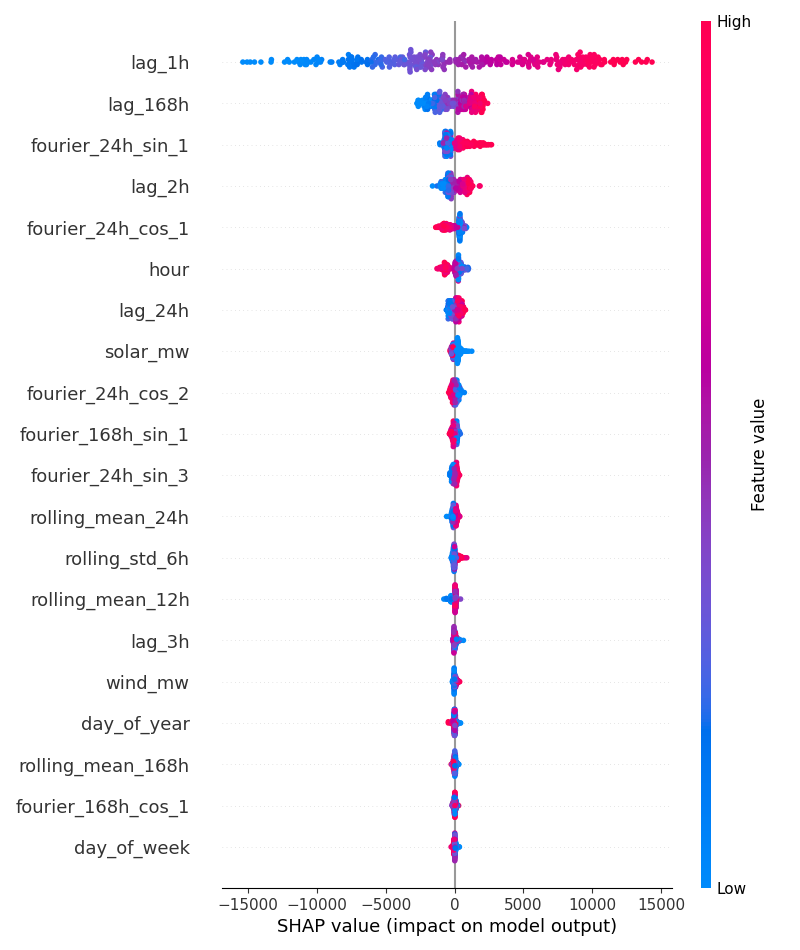
\includegraphics[width=0.55\linewidth]{shap_summary.png}
    \caption{SHAP TreeExplainer summary, 300 validation samples.}
    \label{fig:shap}
\end{figure}

\refstepcounter{section}
\subsection*{C.\quad Great Expectations suite}
\addcontentsline{toc}{subsection}{\protect\numberline{C}Great Expectations suite}
\label{app:ge}

The expectation suite executed by \code{data\_quality} contains the ten expectations listed in Table~\ref{tab:ge}. Structural expectations (column existence, timestamp uniqueness, row count) abort the pipeline on failure; range and null-rate expectations report into the validation JSON without halting.

\begin{table}[H]
\centering
\small
\begin{tabularx}{\linewidth}{@{}l l X@{}}
\toprule
\textbf{Severity} & \textbf{Expectation} & \textbf{Purpose} \\
\midrule
hard     & \code{ExpectColumnToExist}             & Schema integrity (\code{utc\_timestamp}, \code{load\_mw}, \code{wind\_mw}, \code{solar\_mw}). \\
hard     & \code{ExpectColumnValuesToBeUnique}    & Timestamp uniqueness. \\
hard     & \code{ExpectTableRowCountToBeBetween}  & Sanity floor on incoming batch size. \\
hard     & \code{ExpectColumnValuesToBeOfType}    & Numeric types on target and exogenous columns. \\
soft     & \code{ExpectColumnValuesToNotBeNull}   & Bounded null rate per column. \\
soft     & \code{ExpectColumnValuesToBeBetween}   & Load and wind within domain-plausible ranges. \\
\bottomrule
\end{tabularx}
\caption{Great Expectations v1 suite. Hard halts the pipeline; soft only reports.}
\label{tab:ge}
\end{table}

\refstepcounter{section}
\subsection*{D.\quad Key hyperparameters and thresholds}
\addcontentsline{toc}{subsection}{\protect\numberline{D}Key hyperparameters and thresholds}
\label{app:params}

The values in Table~\ref{tab:params} are the parameters in \code{conf/base/parameters.yml} that materially affect the reported numbers. They are deliberately exposed in configuration rather than hardcoded so they can be swept without touching source.

\begin{table}[H]
\centering
\small
\begin{tabularx}{\linewidth}{@{}l l l@{}}
\toprule
\textbf{Group} & \textbf{Parameter} & \textbf{Value} \\
\midrule
Split     & train end                          & 2018-12-31 23:00 \\
          & validation end                     & 2019-12-31 23:00 \\
          & test end                           & 2020-09-30 23:00 \\
LightGBM  & objective                          & \code{regression} (L2) \\
          & num\_leaves                        & 63 \\
          & learning\_rate                     & 0.05 \\
          & colsample\_bytree                  & 0.8 \\
          & subsample                          & 0.8 \\
          & early\_stopping\_rounds            & 50 \\
Quantile  & lower / upper $\alpha$             & 0.1 / 0.9 \\
Conformal & nominal coverage                   & 80\% \\
          & ACI learning rate $\gamma$         & 0.005 \\
CV        & folds                              & 4 (expanding window) \\
Drift     & reference window                   & 2019-01-01 to 2019-06-30 \\
          & clean window                       & 2019-07-01 to 2019-12-31 \\
          & perturb window                     & 2020-03-15 to 2020-05-15 \\
          & Evidently threshold (Wasserstein)  & 0.10 (default) \\
          & concept-drift multiplier           & 1.5 $\times$ baseline median \\
\bottomrule
\end{tabularx}
\caption{Project hyperparameters and thresholds.}
\label{tab:params}
\end{table}

\refstepcounter{section}
\subsection*{E.\quad Concept drift and monthly MAPE}
\addcontentsline{toc}{subsection}{\protect\numberline{E}Concept drift and monthly MAPE}
\label{app:monthly}

Figure~\ref{fig:monthly_mape} shows monthly test MAPE across the 2020 test partition against the median-of-non-perturb-months baseline and the 1.5$\times$ alert threshold. April 2020 is the sole month that breaches the threshold; the detector returns to a quiescent state afterwards, avoiding the persistent false-positive behaviour that would otherwise undermine its operational utility.

\begin{figure}[H]
    \centering
    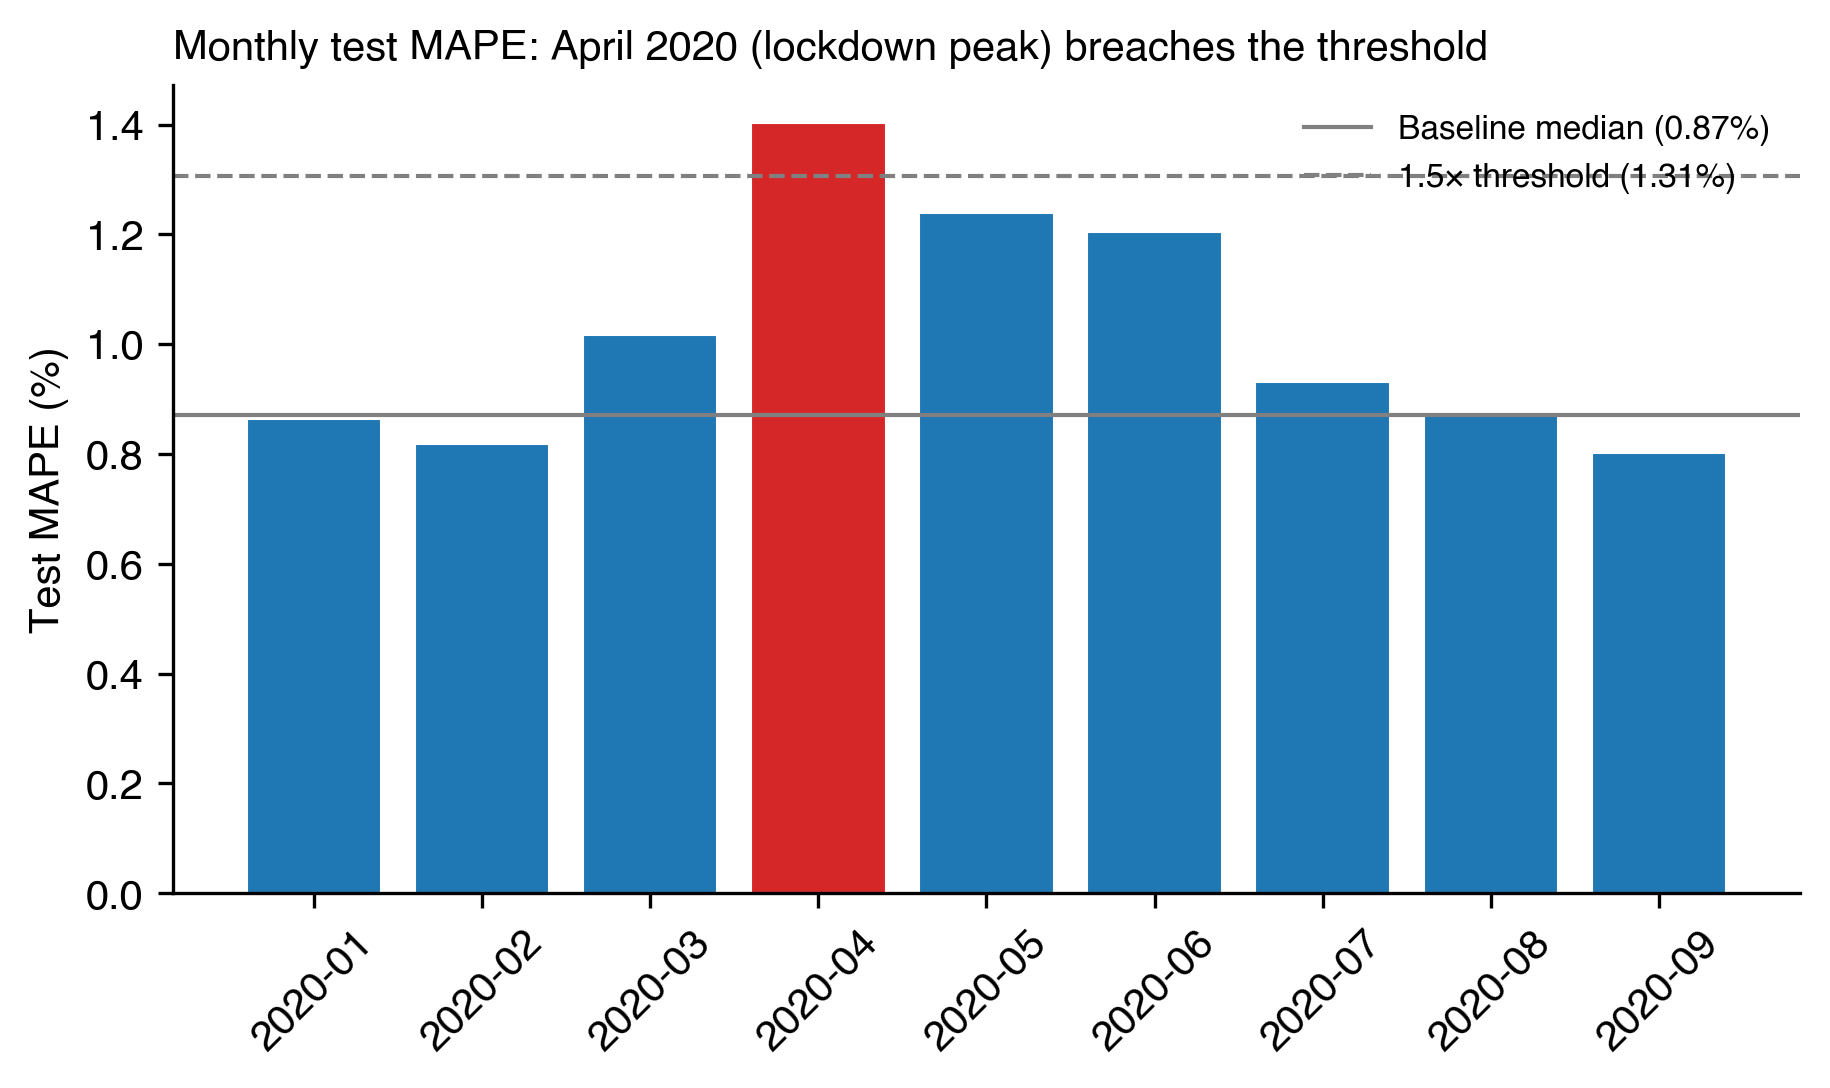
\includegraphics[width=0.7\linewidth]{monthly_mape.png}
    \caption{Monthly test MAPE on the 2020 partition. Baseline 0.87\%, 1.5$\times$ alert 1.31\%.}
    \label{fig:monthly_mape}
\end{figure}

\refstepcounter{section}
\subsection*{F.\quad Prediction-interval calibration breakdown}
\addcontentsline{toc}{subsection}{\protect\numberline{F}Prediction-interval calibration breakdown}
\label{app:pi}

Table~\ref{tab:pi} compares three calibration strategies on the validation and test partitions. Raw quantile heads undercover as expected; split-conformal applies a constant offset of 201~MW to each side and hits the nominal 80\% on validation; ACI further adapts to the test partition at the cost of $\sim$16\% wider intervals.

\begin{table}[H]
\centering
\small
\begin{tabularx}{\linewidth}{@{}l *{4}{>{\centering\arraybackslash}X}@{}}
\toprule
\textbf{Strategy} & \textbf{Val cov.} & \textbf{Val avg width} & \textbf{Test cov.} & \textbf{Test avg width}\\
\midrule
Raw quantile heads ($\alpha = 0.1, 0.9$)        & 64.2\% & 1{,}254~MW & 57.8\% & --- \\
\textbf{Split-conformal} ($Q = 201$~MW, deployed) & \textbf{80.0\%} & \textbf{1{,}656~MW} & \textbf{73.1\%} & \textbf{1{,}611~MW} \\
ACI ($\gamma = 0.005$, sibling log)             & --- & --- & 80.1\% & 1{,}876~MW \\
\bottomrule
\end{tabularx}
\caption{Prediction-interval coverage and average width by strategy.}
\label{tab:pi}
\end{table}

\refstepcounter{section}
\subsection*{G.\quad Packages and versions}
\addcontentsline{toc}{subsection}{\protect\numberline{G}Packages and versions}
\label{app:packages}

The full pinned dependency tree is in \code{pyproject.toml}. The packages that materially affect the reported numbers and the architecture are:

\begin{table}[H]
\centering
\small
\begin{tabularx}{\linewidth}{@{}l l X@{}}
\toprule
\textbf{Component} & \textbf{Version} & \textbf{Role} \\
\midrule
Python                & 3.11                & runtime (CI also covers 3.12) \\
kedro                 & 0.19.8              & pipeline orchestration \\
kedro-mlflow          & 0.14.5              & MLflow integration for Kedro \\
kedro-viz             & 10.2.0              & pipeline visualisation \\
mlflow                & 2.15.1              & experiment tracking and model registry \\
feast                 & 0.58.0              & offline + online feature store \\
great-expectations    & 1.17.1              & data-quality suite \\
evidently             & 0.7.21              & drift detection \\
lightgbm              & 4.6.0               & production regressor (point + quantile heads) \\
prophet               & 1.1.6               & structural-decomposition baseline \\
shap                  & 0.46.0              & TreeExplainer attributions \\
fastapi               & 0.115.0             & serving API \\
uvicorn               & 0.30.6              & ASGI server for FastAPI \\
streamlit             & 1.39.0              & operator dashboard \\
pandas                & 2.2.3               & dataframe handling \\
numpy                 & 1.26.4              & numerical backend \\
scikit-learn          & 1.5.2               & metrics and CV helpers \\
pyarrow               & 17.0.0              & Parquet I/O \\
ruff                  & 0.7.1               & lint + format \\
mypy                  & 1.13.0              & static type checking \\
pytest                & 8.3.3               & test runner \\
pytest-cov            & 6.0.0               & coverage measurement \\
\bottomrule
\end{tabularx}
\caption{Pinned package versions. Full tree in \code{pyproject.toml}.}
\label{tab:packages}
\end{table}

\end{document}
